\chapter{SmartIO}\label{chapter:smartio}
SmartIO is a solution for allowing the local resources of a machine,~i.e., memory and devices, to be shared with and used by remote machines, over standard \gls{pcie}.
%
Our solution works for \emph{all} standard \gls{pcie} devices and their Linux device drivers, no special adaptation is needed in either hardware or software to make this sharing possible.
%
SmartIO is fully distributed and avoids dedicated servers.
%
All machines in the cluster~network may contribute their own local resources and access remote resources.
%
Furthermore, as remote devices and memory resources are accessed over native \gls{pcie}, they can be shared and used by remote machines with very low latency and extremely low computing overhead.
%
Whether devices are actually local or remote becomes irrelevant to the user, as SmartIO eliminates this distinction, with regard to both functionality and performance.
%
In other words, SmartIO is a flexible and efficient solution for scaling out and using more hardware resources than there are available in a single machine.


\section{Underlying idea}\label{sec:idea}
\begin{figure}
    \centering
    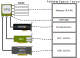
\includegraphics{bus-enumeration}
    \caption[Devices are mapped to the same address space as the \glsfmtshort{cpu} and system memory]
    {Device memory regions (\glsxtrshortpl{bar}) are mapped to the same address space as \glsxtrshort{cpu} and system memory, allowing
    the \gls{cpu} to read from and write to device memory the same way it would access \glsxtrshort{ram}. Devices can similarly use \gls{dma} to read from and write to \glsxtrshort{ram}.}
    \label{fig:bus-enumeration}
\end{figure}
The defining feature of \gls{pcie}~\cite{spec:PCIe} is that devices are mapped into the same address space as the \gls{cpu} and \gls{ram}, as seen in \cref{fig:bus-enumeration}.
%
This allows a \gls{cpu} to read from and write to device memory in the same manner it would access \gls{ram}, also known as \gls{mmio}.
%
Likewise, devices capable of \gls{dma} may read from and write to \gls{ram} directly.
%
\Gls{pcie} also uses \gls{msi}, allowing devices to raise interrupts by writing to an address reserved by the \gls{cpu} instead of requiring dedicated interrupt lines.



This address space mapping occurs when a system enumerates the \gls{pcie} bus and accesses the \gls{cfgspace} of each device.
%
A \gls{cfgspace} contains a description of the capabilities of a device, such as its memory regions.
%
The system will reserve a memory address range for each of these device memory regions, and by writing the start address of these regions to the device's \glspl{bar}, a device is made aware of the address space mapping.
%
Therefore, the term ``\gls{bar}'' is used interchangeably for a region of device memory.
%
Addresses reserved by the system for interrupts are also written to the device's \gls{cfgspace}.
%
For more details on \gls{pcie}, particularly how memory transactions are routed, please refer to \paperref{tocs:pcie,cc:pcie}.



\begin{figure}
    \centering
    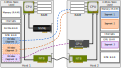
\includegraphics[width=.99\textwidth]{ntb-example}
    \caption[Two computer systems connected using \glsfmtshortpl{ntb}, and the \glsfmtshortpl{ntb} translate between the two different address domains]
    {Two computer systems connected together using \glspl{ntb} and external cables. Host~1 has mapped \glspl{segment} of Host~2's memory through its local \gls{ntb}, providing Host~1 with ``windows'' into the remote system's address space. The \glspl{ntb} translate addresses between the two independent address spaces.}
    \label{fig:ntb-example}
\end{figure}



As depicted in \cref{fig:ntb-example}, it is possible to connect computer systems with different address spaces together over \gls{pcie} by using \glspl{ntb}.
%
\Glspl{ntb} can be embedded as a \gls{cpu} feature~\cite{whitepaper:Sullivan2010,url:LinuxNTB-AMD}, but are more commonly implemented in \gls{pcie} switch chips~\cite{whitepaper:PLX,pex8733}.
%
By using such \gls{ntb}-capable switch chips to implement peripheral devices, independent computer systems can connect with plug-in host adapter cards and external cables.
%
To the system, the \gls{ntb} appears as a normal \gls{pcie} device\footnote{The \gls{pcie} terminology for individual \glspl{devicefunction} is ``\glspl{ep}''. We use the terms ``device'' and ``\gls{function}'' as synonyms for a \gls{pcie} \gls{ep} throughout this dissertation.} with one or more \glspl{bar} that are reserved and mapped during the enumeration process.
%
However, rather than being backed by device registers or device memory, the \gls{ntb} instead forwards reads and writes to its \glspl{bar} from one side of the \gls{ntb} to the other, translating memory addresses in the process.
%
The \gls{ntb} uses a \gls{lut} for address translation, which can be configured dynamically during run-time.
%
By using different base offsets in this \gls{lut}, it is possible to configure several memory-mappings (or ``windows'') into the address space of a remote system.
%
\Cref{fig:ntb-example} illustrates how arbitrary memory addresses on the remote system can be mapped, allowing the local \gls{cpu} to access remote memory as if it was local device memory.
%
Although address translation between the different address spaces is very fast since the \gls{lut} is implemented in \gls{ntb} hardware, the number of \gls{ntb} windows is limited by the maximum number of table entries.
%
More details on how \glspl{ntb} work can be found in \paperref{tocs:pcie-ntb}.



Since device memory on a remote system is part of the same address space as system memory, we can use an \gls{ntb} to map memory of a remote device.
%
We show this in \cref{fig:ntb-example}, where Segment~3 is allocated in \gls{gpu} memory rather than system~\gls{ram}, but still mapped for the \gls{cpu} of Host~1's similarly to the other \glspl{segment}.
%
By mapping all \glspl{bar} of a remote device for a local \gls{cpu}, it would be possible to perform memory operations on the remote device, such as reading from or writing to device registers.
%
Moreover, device~\gls{dma} is not limited to reading and writing to system \gls{ram}, but can also be used to access memory on other devices in the same address space.
%
This is known as ``\gls{p2p}'' in \gls{pcie}, and provides us with an opportunity as it becomes possible for a device to read and write directly across an \gls{ntb}.
%
We can use this to map memory resources for a device, be it \gls{ram} or memory of other devices. 
%
Furthermore, because \gls{pcie} uses \gls{msi}, it is even possible to map interrupt addresses through an \gls{ntb}, as they too are mappable.




\section{Main challenges}\label{sec:challenges}
Although \glspl{ntb} provide the fundamental memory mapping capabilities that can facilitate the use of remote devices, the challenge is to avoid requiring device drivers to be aware of remote-side address spaces.
%
As touched upon in \cref{sec:motivation}, this is desirable in order to use existing device driver implementations.
%
In order for a device driver running on a local~machine to use a remote~device, we must make sure that the driver uses addresses that is mapped through both the local and remote \glspl{ntb}.
%
For instance, when the device driver attempts to access \glspl{devicebar}, we must make sure that the driver uses memory addresses that are mapped through the local, or \gls{cpu}-side, \gls{ntb} without the driver or device being aware of this.
%
Conversely, when the device driver attempts to initiate \gls{dma} transfers or configures an interrupt vector address, we must find a way to transparently inject memory addresses that are mapped through the remote, or device-side, \gls{ntb}.



One possibility is to use virtualization to mitigate the complexity of managing different address spaces.
%
The fact that devices are on the other side of an \gls{ntb} could be hidden for device drivers by distributing devices to \gls{vm} \glspl{guest} instead of physical \lgls{host}{host~machines}.
%
The \gls{hypervisor} on a \lgls{host}{host~machine} can be modified to assist setting up necessary \gls{ntb} (and \gls{iommu}) mappings to the respective device memory and \gls{vm} memory.
%
This would make it possible to \gls{passthrough} a remote device to a \gls{vm} \gls{guest} running on a local \lgls{host}{host~machine}.
%
However, requiring that compute tasks run in \glspl{vm} limits the generality of a solution.
%
Virtualization is not necessarily appropriate in all circumstances, as it may add additional system load because \gls{cpu} cycles are spent on \lgls{host}{hosting} the virtualized environment.
%
A more general mechanism is needed for abstracting away the complexity of dealing with a remote-side address space, which can be used to support sharing for \glspl{vm} and bare-metal machines alike.



\Gls{dma} is particularly challenging in this context.
%
A device driver running on the \gls{hostmachine} may assume that any local memory address can be reached by the device, but as explained in \cref{sec:idea}, the \gls{ntb} only provide \emph{windows} into a remote address space.
%
It is generally not possible to predict in advance which memory addresses a device driver may use, yet memory must be mapped through the \gls{ntb} before the driver initiates \gls{dma} transfers.
%
This is not solved by virtualization either, as \gls{passthrough} is faced with the same problem:
%
a device driver running in the \gls{vmguest} will be both unaware of the fact that it is running in an virtualized address space \emph{and} that the device is on the other side of an \gls{ntb}, and may try to use any (virtualized) memory address.
%
The only solution is to map the entire memory of the \gls{guest}, but this requires a mechanism to detect \gls{hostphys} memory used by the \gls{emulator} so that it may be mapped through the \gls{ntb}.
%
Additionally, a mechanism for discovering the virtual, or \gls{guestphys}, memory layout of the \gls{vm} is also needed, so that the device can be mapped to the same virtual address space as the \gls{vm}.



Another consideration is the performance.
%
Deferring the action of mapping memory through the \gls{ntb} until a device driver initiates \gls{dma}, or some other time when the specific addresses of \gls{dma} buffers and \gls{vm} memory can be known, is not viable;
%
synchronizing with the remote system at this time will introduce communication overhead in the performance-critical path.
%
The naive solution is to map the entire system memory (of the \gls{hostmachine}) for the device, but this workaround requires the \gls{ntb}~\glspl{bar} to be at least \emph{as large} as the size of \gls{ram}.
%
This does not scale very well, as it would effectively limit the number of machines the cluster can support;
%
each machine added would increase the \gls{ntb} memory requirements by its entire \gls{ram} size.
%
Moreover, the number of maps supported by an \gls{ntb} is also limited (by the size of its \gls{lut}).
%
We must find a way to prepare memory-maps through the \gls{ntb} in advance of use, in order to avoid adding communication latency in the critical path, and without requiring that the entire \gls{host} memory is mapped for the device.




The published papers provide further details on these challenges as part of the description of the implementation of the different components of SmartIO.
%
Particularly \paperref{tocs:lending,tocs:mdev,tocs:nvme} provide a more in-depth explanation of what the main challenges are, and they also explain how SmartIO tackle them.
%
A discussion of additional considerations is given in \paperref{tocs:disc}.




\section{Implementation}\label{sec:implementation}
In our framework, computer systems act as \emph{``\glspl{borrower}''} and \emph{``\glspl{lender}''}.
%
A \gls{lender} is a computer system that registers one or more of its internal \gls{pcie} devices with SmartIO, allowing these devices to be distributed to and used by remote machines.
%
A \gls{borrower} is a system that is currently using such a device. 
%
While a device only has one \gls{lender}, namely the computer system where it is physically installed, there can be several \glspl{borrower} using it simultaneously.
%
SmartIO also makes it possible for a system to act as both \gls{lender} and \gls{borrower} at the same time, lending out its own local devices and simultaneously borrowing remote devices from other machines.



Basing our framework on standard \gls{pcie} is a a crucial part of the design.
%
Not only does this allow commodity devices to be operated remotely by standard device drivers over native \gls{pcie}, but this design also means that the implementation complexity of SmartIO lies entirely in software.
%
In fact, SmartIO can be implemented for existing computer systems that are connected using \glspl{ntb} in any network topology, regardless of whether the \glspl{ntb} are switch chips soldered onto a motherboard~(part of a ``system-on-chip'') or implemented as plug-in adapter cards.



Unlike other solutions for distributed \gls{io}, SmartIO combines traditional \gls{io} with distributed shared-memory functionality in a seamless manner.
%
Sharing is supported at multiple abstraction levels:
%
devices may be distributed to physical \glspl{hostmachine} and to \glspl{vm} alike.
%
Individual \lgls{function}{device functions} of \lgls{function}{multi-function} devices may be distributed to different machines in the network, or to the same machine should it require multiple resources.
%
SmartIO also provides software facilities for \gls{disaggregating} devices and memory resources, allowing device drivers to be implemented as part of distributed cluster applications or other \gls{userspace} applications. 
%
This makes it possible for several machines to simultaneously share a single \lgls{function}{device~(function)}.
%
It is even possible to \emph{combine} the sharing methods of SmartIO. 
%
For example, we can \gls{disaggregate} the device memory of a remote \gls{gpu} while it is being borrowed using the \gls{apiext}, or we can share \glspl{vf} of an \gls{sriov} \gls{nic} with both physical \glspl{hostmachine} and \glspl{vm}.


\begin{figure}
    \centering
    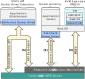
\includegraphics{software-architecture}
    \caption[Three different sharing methods are made possible by our framework. The SmartIO driver abstracts away the physical location of a remote resource]
    {The software architecture of SmartIO. Three different sharing methods are made possible by our framework: \textbf{(1)}~\gls{dl}, \textbf{(2)}~\gls{mdev}, and \textbf{(3)}~using the \gls{sisciapiext}. The SmartIO driver, shown as \textbf{(B)}, abstracts away the physical location of remote resources, for both the shared device and software using the device.}
    \label{fig:architecture}
\end{figure}


In this section we address the challenges of \cref{sec:challenges}, and give a bottom-up summary of the implementation of SmartIO.
%
\cref{fig:architecture} illustrates the different components of our framework, and how they fit together.
%
The full implementation details can be found in the published papers, with \cref{paper:tocs} providing a detailed description of the entire solution as a whole.



\subsection{Low-level NTB driver}\label{sec:ntb-driver}
SmartIO is implemented on top of the \gls{ntb} interconnection solution from Dolphin.
%
The low-level \gls{ntb} driver, illustrated as layer \textbf{(A)} in \cref{fig:architecture}, provides the fundamental \gls{pcie} networking infrastructure and memory mapping functionality which SmartIO builds on.
%
Individual systems may contribute parts, or \emph{``\glspl{segment}''}, of their local memory to a distributed, shared memory space. 
%
\Glspl{memorysegment} in remote machines may be mapped into the local address space of a system by using the \gls{ntb}, as explained in \cref{sec:idea}.
%
Moreover, \gls{userspace} applications may use the \gls{sisciapi} to interact with the \gls{ntb} driver to manage \glspl{memorysegment} and implement shared-memory communication.



\subsection{SmartIO driver}\label{sec:smartio-driver}
The SmartIO driver, shown as layer \textbf{(B)} in \cref{fig:architecture}, runs on all machines in the cluster.
%
It acts as an abstraction layer, providing a logical decoupling of devices and which physical machines, or \emph{\glspl{lender}}, they are installed in.
%
Neither devices nor software need to consider where resources physically reside, since SmartIO resolves this on behalf of both devices and a machines using them, or \emph{\glspl{borrower}}.


Devices registered with SmartIO are assigned an unique identifier which allows machines to refer to a device without needing to specify the \gls{lendermachine}.
%
Internally, the SmartIO driver keeps track of devices and \glspl{lender}, and uses this device identifier to look up machines, devices, and which \gls{ntb} to use.
%
The SmartIO driver is also responsible for making \glspl{devicebar} available as \glspl{sharedsegment}, making it possible for \glspl{borrowermachine} to memory map remote device memory into their local address space (\gls{mmio}).



Most important is the SmartIO driver's responsibility of mapping \glspl{memorysegment} \textbf{on behalf of a device} and returning \gls{io} addresses to these maps, \textbf{as seen by the device}.
%
The SmartIO driver works out the physical locations of devices and \glspl{memorysegment},~i.e., which machines they reside in and which \glspl{ntb} a device must use in order to reach a \gls{segment}.
%
Note that a \gls{segment} can reside in memory of the machine using the device~(the \gls{borrower}), in memory of the machine where the device is installed~(the \gls{lender}), or a different cluster machine altogether.
%
\Glspl{borrower} are not required to know anything about \gls{io} addresses returned by our SmartIO driver, other than the fact that they resolve to the same address space as the device.
%
This allows both a \gls{borrower} and the device to remain agnostic about the underlying, physical \gls{pcie} topology, as they can rely on the SmartIO driver to resolve paths in the cluster network and map resources through the appropriate \glspl{ntb}.



The SmartIO driver solves the challenge of managing multiple address spaces, as described in \cref{sec:challenges}.
%
For example, a \gls{borrower} can request a \gls{memorysegment} in a different machine is mapped so that the device may use \gls{dma} to it.
%
Our SmartIO driver will look up the \gls{lendermachine} and which (device-side) \gls{ntb} it must use, configure the \gls{ntb}, map the \gls{memorysegment} for the device, and return the (device-side) \gls{io} address of this map back to the \gls{borrower}.
%
The \gls{borrower} can then use this \gls{io} address when interacting with the device in order to initiate the \gls{dma} transfer, and the device is able to reach the \gls{memorysegment} through the lender's \gls{ntb}.
%
\Glspl{borrower} do not need to be aware of the internal \gls{io} address space layout of a \gls{lender}.
%
As it happens, they do not even need to know which physical machine the \gls{lender} is.



With the abstraction the SmartIO driver provides, our framework is able to facilitate the sharing and use of remote resources (both memory and devices) as described in \cref{sec:lending,sec:mdev,sec:api}.
%
More details on how SmartIO resolves the paths between devices and other memory resources that must be mapped (for devices) are given in the papers, particularly in \paperref{tocs}.
%
However, please note that the SmartIO driver is not mentioned explicitly by name in the papers, as the description of its functionality is interleaved with the implementation details of the sharing methods of SmartIO,~i.e., \gls{dl}, \gls{mdev}, and the \gls{apiext}.



\subsection{Device Lending}\label{sec:lending}
\Gls{dl}, illustrated as arrow \textbf{(1)} in \cref{fig:architecture}, makes it possible to share and distribute devices to remote \glspl{hostmachine}.
%
The devices become part of the system they are shared with, allowing application software, device drivers, and even the \gls{os} to use them as if they were locally installed.
%
While \gls{dl} only allows individual \glspl{devicefunction} to be distributed to a single machine at the time, it is nevertheless highly suitable in the case where a device has a complex or proprietary device driver as no modifications to existing software is required.


As mentioned in \cref{sec:idea}, it is possible to map the device memory regions, or \glspl{bar}, of a remote device through an \gls{ntb}.
%
Using the \gls{ntb}, a local \gls{cpu} can perform memory operations on a remote device, such as reading from and writing to device registers.
%
Conversely, local resources, such as \gls{ram} and interrupt addresses, can in turn be mapped for the remote device itself. 
%
This allows the remote device to use \gls{dma} through the \gls{ntb} and trigger interrupt routines on the local \gls{cpu}.
%
The SmartIO driver, as explained in \cref{sec:smartio-driver}, eliminates the complexity of managing multiple address spaces: a user may rely on the SmartIO driver to map resources through the appropriate \glspl{ntb} and provide \gls{io} addresses corresponding to a device's address space.
%
However, as pointed out in \cref{sec:challenges}, we still need to make sure that device drivers use this functionality without requiring that they be re-written. 
%
More precisely, we need a mechanism for transparently injecting resolved \gls{io} addresses, without the devices or their drivers being aware of this.



\begin{figure}
    \centering
    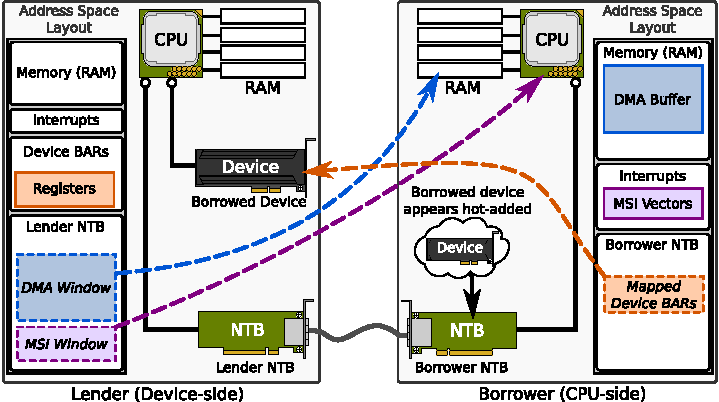
\includegraphics[width=.99\textwidth]{device-lending}
    \caption
    [The memory regions of a remote device is mapped for the \glsfmtshort{cpu} on the borrower, so that it can read and write to device registers. Local resources are mapped for the device, so that it may use \glsfmtshort{dma} and trigger interrupts. \Glsentrytext{dl} inserts a \glsentrytext{shadowdev} into the local device tree using these mappings, making remote device access transparent to both \glsfmtshort{cpu} and device.]
    {The memory regions of a remote device is mapped for the \gls{cpu} on the borrower, so that it can read and write to device registers. Local resources are mapped for the device, so that it may use \gls{dma} and trigger interrupts. \Gls{dl} inserts a \gls{shadowdev} into the local device tree using these mappings, making remote device access transparent to both \gls{cpu} and device.}
    \label{fig:device-lending}
\end{figure}


\Gls{dl} solves this by inserting a ``\gls{shadowdev}'' into the local \gls{pcie} device tree on the \gls{borrower}, as depicted in \cref{fig:device-lending}. 
%
The \gls{shadowdev} makes it appear as if the remote device has been \gls{hotadded} to the local system, and provides us with a mechanism for intercepting interactions with the device by the \gls{os} and any device drivers. 
%
We make sure that a device driver attempting to memory map the device's \glspl{bar} use addresses that map through the \gls{ntb}, without the driver being aware that the device is actually remote.
%
Similarly, when the device driver configures interrupts, we are able to intercept this and inject an address that map through the \gls{lender}'s \gls{ntb}, again without the driver being aware.



\begin{figure}
    \centering
    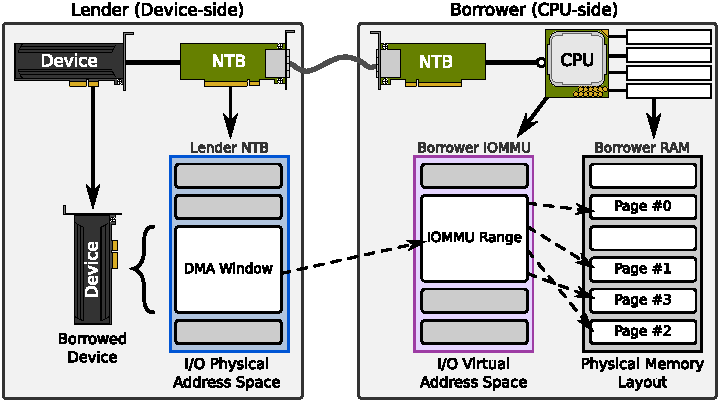
\includegraphics[width=.99\textwidth]{dma-window}
    \caption[The borrower's \glsfmtshort{iommu} is used to create a single continuous memory range that may be mapped through the lender's \glsfmtshort{ram}. Adding and removing memory pages from the local \glsfmtshort{iommu} group is inexpensive compared to actively communicating with the remote lender~machine in order to map dynamically]
    {The \gls{borrower}'s \gls{iommu} is used to create a single continuous memory range that may be mapped through the \gls{lender}'s \gls{ntb}, in order for the remote device to reach local \gls{ram}. Adding and removing memory pages from the local \gls{iommu} group is inexpensive compared to actively communicating with the remote \gls{lendermachine} in order to map dynamically.}
    \label{fig:dma-window}
\end{figure}


The \gls{shadowdev} also provides us with the means to detect when a device driver is allocating \gls{dma} buffers and making memory available for \gls{dma} transfers.
%
Notwithstanding, unlike \glspl{devicebar} and \gls{msi} addresses, memory addresses for \gls{dma} buffers are not known in advance, as mentioned in \cref{sec:challenges}.
%
Mapping \glspl{bar} and interrupts is a one-time operation.
%
The pages used for \gls{dma} memory buffers, on the other hand, may be scattered in physical memory.
%
A driver may even initiate several transfers to different parts of memory altogether.
%
Mapping individual memory pages through the \gls{lender}'s \gls{ntb} would not only exhaust the number of available entries in its \gls{lut}, but communicating with the \gls{lendermachine} in order to map these pages dynamically would introduce communication latency in the critical performance path.



To solve this, \gls{dl} relies on the \gls{iommu} on the \gls{borrower} as depicted in \cref{fig:dma-window}.
%
We can prepare a contiguous memory address range \emph{in advance} using the \gls{borrower}'s \gls{iommu}.
%
This range can be mapped through the \gls{lender}'s \gls{ntb} with a single map, or ``\gls{dmawindow}'', even before any device drivers are using the device.
%
When a device driver, at a later point, allocates \gls{dma} buffers, we can simply add these addresses to the \gls{iommu} range.
%
Since this is an entirely local operation (on the \gls{borrower}), communication with the remote \gls{lendermachine} is avoided.
%
Moreover, all address translations between the different address domains are done in \gls{ntb} and \gls{iommu} hardware, ensuring that this solution is able to achieve native \gls{pcie} performance in the data path.



A more technical description of the implementation of \gls{dl} can be found in \paperref{tocs:lending}, including details about the \gls{shadowdev} and \glspl{cfgcycle}.
%
\paperref{tocs:lending-p2p,cc:p2p} explain how \gls{dl} is able to support \gls{p2p} \gls{dma} between multiple borrowed devices, even when they reside in different \glspl{lendermachine}.
%
In addition, \paperref{tocs:lending-dma,tocs:disc-devs} explain how we can use the \emph{\gls{lender}'s} \gls{iommu} to remap \glspl{dmawindow} from high to low memory addresses for devices with addressing limitations.



\subsection{MDEV}\label{sec:mdev}
Our \gls{mdev} implementation, shown as arrow \textbf{(2)} in \cref{fig:architecture}, enables the Linux~\gls{kvm} to ``\emph{\lgls{passthrough}{pass through}}'' borrowed devices to \glspl{vm}.
%
This \gls{passthrough} makes it possible for software running in a \gls{vmguest} to use the physical device directly, without compromising the memory isolation provided by the virtualization.
%
As devices are no longer tightly coupled with the \glspl{hostmachine} they are installed in, \gls{mdev} makes it possible to distribute \glspl{vm} across different \glspl{host} in the cluster while benefiting from the bare-metal performance of direct access to physical hardware.

\begin{figure}
    \centering
    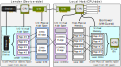
\includegraphics[width=.99\textwidth]{mdev-dma}
    \caption{MDEV}
    \label{fig:mdev-dma}
\end{figure}

\begin{itemize}
    \item \textbf{very} brief: what is passthrough/VFIO
    \item what MDEV gives us
    \item how to map VM memory for device
    \item relaying interrupts (see papers)
    \item busmaster hack
    \item probing memory layout
\end{itemize}

\subsection{API extension}\label{sec:api}
\begin{itemize}
    \item why do we need API? (disaggregation in software + shared memory networking)
    \item short explanation of SISCI
    \item what functions did we add to SISCI?
\end{itemize}



\subsection{NVMe driver}\label{sec:nvme}
\begin{itemize}
    \item why a prototype driver? demonstrate disaggregation in software
    \item why nvme? easy to parallelize because of queues
    \item driver implementation and queue sharing
    \item gpudirect + co-operation with device lending
\end{itemize}

%\section{Workload}\label{sec:eval}

\section{Performance measurements}\label{sec:eval}
Some selected performance graphs here, demonstrating zero-overhead :)

\section{Related work}\label{sec:rw}
should rw go in discussion and conclusion instead?
\begin{itemize}
    \item rdma stuff
    \item fabric partitioning: mr-iov, broadcom/microsemi chips with partitioning
    \item ladon (and other ntb stuff)
    \item disaggregation
\end{itemize}

\glspl{guest}

% RW first??
%An example of this is rCUDA, where multiple clients may run jobs on the same \gls{gpu} by relying ~\cite{Duato2010}
%\Gls{rdma}-based \gls{disaggregation} can even allow a single resource to be shared by several machines in the cluster at the same time. 
%
%However, since 
%Our solution provides a more general mechanism for abstracting away the complexity of dealing with a remote-side address space, without relying on \glspl{vm}.
%
%Using SmartIO, it becomes possible to distribute devices to bare-metal machines, while still allowing device drivers and even the \gls{host}~\gls{os} to remain unaware of remote address spaces.
%
%Nonetheless, \gls{passthrough} to \glspl{vm} is \emph{also} possible using our implementation.
%
%Furthermore, our framework is able to prepare \gls{ntb} windows in advance of use.
%
%This way, we avoid communicating with remote machines in the critical path, allowing \gls{dma} addresses to be transparently injected without incurring any performance overhead.
%
%With SmartIO, the hard separation between local and remote is blurred, as remote resources may be used as if they were locally installed and with native \gls{pcie} performance.




%without requiring software to be aware of the underlying, physical \gls{pcie} topology or the internal \gls{io} address space layout of remote machines.
%
%The SmartIO driver is able to resolve the \gls{lender} and 
%
%
%        %
%        Furthermore, our SmartIO driver also supports setting up mappings between multiple devices, even when they reside in different \glspl{lender}, allowing \gls{pcie} transactions between them to be routed along the shortest path in the cluster network (\gls{p2p}).
%
%is then announced to other machines in the cluster~network. 
%%
%Different machines can use this
%This identifier allows different machines to refer to a device, without needing to specify which machine it resides in.
%%
%
%
%which allows different machines to refer to a device without 
%
%%%% TODO FIXME NOTE: Pål wanted to end this section with a paragraph on "this is how we do it" or "we support X or Y" or something like this
%% the idea of the smartio driver should go here, i.e., mapping segments on behalf of the device, using global/cluster identifiers etc.
%% use "layer" etc
%% still direct access to hw when mappings are in place
%
%agnostic about remote address space.
%and is responsible for dynamically setting up \gls{ntb} mappings, translating addresses between different address spaces, and resolving paths in the cluster.
%
%%SmartIO solves these issues by logical decoupling devices and the physical machines they are installed in.
%%%
%%When devices are registered with our framework, they are assigned an unique identifier.
%%
%%
%%%In SmartIO, we solve this ... 
%%\begin{itemize}
%%    \item device identifier
%%    \item resolve adapters/paths
%%    \item mapping on behalf of device
%%    \item briefly mention shadow device for intercepting
%%    \item DMA windows
%%\end{itemize}
%
%
%Illustrated as layer {\textsf{(A)}} in \cref{fig:architecture}.
%        %
%
%    %\item[SmartIO Driver] Illustrated as layer {\textsf{(B)}} in \cref{fig:architecture}.
%        %
%        %
%        %
%
%    %\item[Device~Lending] Illustrated by arrow {\textsf{(1)}} in \cref{fig:architecture}.
%        Device~Lending allows devices to be time-shared among machines in the network.
%        %
%        Remote devices can be dynamically added to a system while it is running and inserted into the local \gls{pcie} device tree of a machine.
%        %
%        When the system performs configuration cycles or allocates \gls{dma} buffers, SmartIO intercepts this and inject remote addresses in a transparent manner.
%        %
%        This allows existing software to use a remote device without requiring any modifications or special adaptions;
%        device drivers, applications software, and even the \gls{os} can use the device as if it was locally installed.
%        %
%
%    %\item[\gls{mdev}] Illustrated by arrow {\textsf{(2)}} in \cref{fig:architecture}.
%        %
%        The \gls{mdev} extension to the \gls{kvm} facilitates \gls{passthrough} of borrowed devices to \glspl{vm}.
%        %
%        \Glspl{vmguest} can access these remote devices directly, without breaking out of the memory isolation provided by the virtualization.
%        %
%        \Gls{mdev} makes it possible for \glspl{vm} to be distributed on different \glspl{host} in the cluster while benefiting from the bare-metal performance of direct access to physical hardware.
%
%    %\item[\gls{api} Extension] Illustrated by arrow {\textsf{(3)}} in \cref{fig:architecture}.
%        %
%        As an alternative to Device~Lending and \gls{mdev}, our SmartIO solution also provides an extension to the \gls{sisciapi} for managing devices and developing (distributed) device drivers.
%        %
%        This includes functionality for memory-mapping device registers and mapping shared memory segments for a device.
%        %
%        Our \gls{api}~extension makes it possible for device operation to become part of the cluster application itself, allowing devices to access shared memory segments using native \gls{dma}.
%        %
%        By relying on our SmartIO framework to resolve memory addresses between individual address spaces, a driver implementation does not need to consider the system-local address space of the machine where the device is installed.
%        %
%        This greatly reduces the complexity of implementing distributed applications, as it becomes possible for software to assume that \gls{io} resources are local, while taking full advantage of shared-memory capabilities.
%        %
%        Using this \gls{api}~extension, devices may be \gls{disaggregated} at the software level and shared simultaneously between application processes running on different remote machines.
%%
%
%
%%Need a concluding sentence leading to the further descriptions of the various components below.
%
%% something about direct access?
%
%



%%
%Also unlike existing \gls{pcie}-based solutions, SmartIO is fully distributed and avoids dedicated servers.
%All machines in the cluster can contribute their own local resources and access remote resources, even at the same time.
%%
%Finally, by using \gls{pcie} shared memory techniques, SmartIO is able to abstract away the physical location of devices and memory resources. 
%Memory addresses are translated between different address domains by SmartIO in a manner that is transparent to application software, device drivers, and even the \gls{os}.
%This makes it possible to provide optimizations based on resource locality and minimizing data movement, without requiring the user to be aware of the underlying PCIe topology.
%\section{General idea}\label{sec:idea}

%    \item \textbf{Address resolution mechanism}: 
%        SmartIO provides functionality for 
%        
%
%        %
%        this makes it possible to abstracting away the physical location of devices and memory segments,~i.e., which machines they are installed in.
%
%        %
%        functionality for transparently translating \gls{io} addresses between th different address spaces
%
%        and is able to abstract away the location of devices and memory segments,~i.e., which machines they are installed in.
%
%        (or device-side) addresses.
%        %
%        With this abstraction, SmartIO facilitates the use of remote resources (both memory and devices) without requiring the user to be aware of the underlying, physical \gls{pcie} topology or the internal \gls{io} address space layout of remote machines.
%        %
%        Furthermore, this mechanism is also able to support mapping 
%
%        SmartIO provides a logical decoupling of devices and which physical machines they are installed in on several abstraction levels.
%%
